% ------------------------------------------------------------------------
% ------------------------------------------------------------------------
% abnTeX2: Modelo de Trabalho Academico (tese de doutorado, dissertacao de
% mestrado e trabalhos monograficos em geral) em conformidade com 
% ABNT NBR 14724:2011: Informacao e documentacao - Trabalhos academicos -
% Apresentacao
% ------------------------------------------------------------------------
% ------------------------------------------------------------------------

\documentclass[
    % -- opções da classe memoir --
    12pt,               % tamanho da fonte
    openright,          % capítulos começam em pág ímpar (insere página vazia caso preciso)
    oneside,
    %twoside,           % para impressão em recto e verso. Oposto a oneside
    a4paper,            % tamanho do papel. 
    % -- opções da classe abntex2 --
    %chapter=TITLE,     % títulos de capítulos convertidos em letras maiúsculas
    %section=TITLE,     % títulos de seções convertidos em letras maiúsculas
    %subsection=TITLE,  % títulos de subseções convertidos em letras maiúsculas
    %subsubsection=TITLE,% títulos de subsubseções convertidos em letras maiúsculas
    % -- opções do pacote babel --
    english,            % idioma adicional para hifenização
    french,             % idioma adicional para hifenização
    spanish,            % idioma adicional para hifenização
    brazil              % o último idioma é o principal do documento
    ]{abntex2}

% ---
% Pacotes básicos 
% ---
\usepackage{lmodern}            % Usa a fonte Latin Modern          
\usepackage[T1]{fontenc}        % Selecao de codigos de fonte.

\usepackage{lastpage}           % Usado pela Ficha catalográfica
\usepackage{indentfirst}        % Indenta o primeiro parágrafo de cada seção.
\usepackage{color}              % Controle das cores
\usepackage{graphicx}           % Inclusão de gráficos
\usepackage{microtype}          % para melhorias de justificação
\usepackage{longtable}          % para tabelas longas
\usepackage{multirow}
\usepackage{algpseudocode,algorithm}    % para algoritmos       
\usepackage{pdfpages}
\usepackage{subfig}
\usepackage{hyperref}
\usepackage{amsmath}
%\usepackage{subcaption}
% ---
        
% ---
% Pacotes adicionais, usados apenas no âmbito do Modelo Canônico do abnteX2
% ---
\usepackage{lipsum}             % para geração de dummy text
% ---

% ---
% Pacotes de citações
% ---
\usepackage[brazilian,hyperpageref]{backref}     % Paginas com as citações na bibl
\usepackage[alf]{abntex2cite}   % Citações padrão ABNT

% --- 
% CONFIGURAÇÕES DE PACOTES
% --- 

% ---
% Configurações do pacote backref
% Usado sem a opção hyperpageref de backref
\renewcommand{\backrefpagesname}{Citado na(s) página(s):~}
% Texto padrão antes do número das páginas
\renewcommand{\backref}{}
% Define os textos da citação
\renewcommand*{\backrefalt}[4]{
    \ifcase #1 %
        Nenhuma citação no texto.%
    \or
        Citado na página #2.%
    \else
        Citado #1 vezes nas páginas #2.%
    \fi}%
% ---

% ---
% Informações de dados para CAPA e FOLHA DE ROSTO
% ---
\titulo{Uso da Técnica EbE-FEM para a solução em GPU de um problema do eletromagnetismo}
\autor{Thiago de Sousa Goveia}
\local{Timóteo}
\data{2017}
\orientador{Márcio Matias}
\coorientador{Lucas Pantuza Amorim}
\instituicao{%
    Centro Federal de Educação Tecnológica de Minas Gerais
    \par
    Campus Timóteo
    \par
    Graduação em Engenharia de Computação
}
\tipotrabalho{Trabalho de conclusão de curso (Graduação)}

% O preambulo deve conter o tipo do trabalho, o objetivo, 
% o nome da instituição e a área de concentração 
\preambulo{Monografia apresentada à Coordenação de Engenharia de Computação do Campus Timóteo do Centro Federal de Educação Tecnológica de Minas Gerais para obtenção do grau de Bacharel em Engenharia de Computação.}
% ---


% ---
% Configurações de aparência do PDF final

% alterando o aspecto da cor azul
\definecolor{blue}{RGB}{41,5,195}

% informações do PDF
\makeatletter
\hypersetup{
        %pagebackref=true,
        pdftitle={\@title}, 
        pdfauthor={\@author},
        pdfsubject={\imprimirpreambulo},
        pdfcreator={LaTeX with abnTeX2},
        pdfkeywords={abnt}{latex}{abntex}{abntex2}{trabalho acadêmico}, 
        colorlinks=true,            % false: boxed links; true: colored links
        linkcolor=blue,             % color of internal links
        citecolor=blue,             % color of links to bibliography
        filecolor=magenta,              % color of file links
        urlcolor=blue,
        bookmarksdepth=4
}
\makeatother
% --- 

% --- 
% Espaçamentos entre linhas e parágrafos 
% --- 

% O tamanho do parágrafo é dado por:
\setlength{\parindent}{1.3cm}

% Controle do espaçamento entre um parágrafo e outro:
\setlength{\parskip}{0.2cm}  % tente também \onelineskip

% ---
% compila o indice
% ---
\makeindex
% ---

% ----
% Início do documento
% ----
\begin{document}

% Seleciona o idioma do documento (conforme pacotes do babel)
%\selectlanguage{english}
\selectlanguage{brazil}

% Retira espaço extra obsoleto entre as frases.
\frenchspacing 

% ----------------------------------------------------------
% ELEMENTOS PRÉ-TEXTUAIS
% ----------------------------------------------------------
% \pretextual

% ---
% Capa
% ---
\imprimircapa
% ---
% ---
% Folha de rosto
% (o * indica que haverá a ficha bibliográfica)
% ---
\imprimirfolhaderosto
% ---

% ---
% Inserir folha de aprovação
% ---

% Isto é um exemplo de Folha de aprovação, elemento obrigatório da NBR
% 14724/2011 (seção 4.2.1.3). Você pode utilizar este modelo até a aprovação
% do trabalho. Após isso, substitua todo o conteúdo deste arquivo por uma
% imagem da página assinada pela banca com o comando abaixo:
%
% \includepdf{folhadeaprovacao_final.pdf}
%
\begin{folhadeaprovacao}

  \begin{center}
    {\ABNTEXchapterfont\large\imprimirautor}

    \vspace*{\fill}\vspace*{\fill}
    \begin{center}
      \ABNTEXchapterfont\bfseries\Large\imprimirtitulo
    \end{center}
    \vspace*{\fill}
    
    \hspace{.45\textwidth}
    \begin{minipage}{.5\textwidth}
        \imprimirpreambulo
    \end{minipage}%
    \vspace*{\fill}
   \end{center}
        
   Trabalho aprovado. \imprimirlocal, 07 de abril de 2017:
   
   \assinatura{\textbf{Prof. \imprimirorientador} \\ Orientador} 
   \assinatura{\textbf{Prof. Marcelo de Sousa Balbino} \\ Coorientador}
   \assinatura{\textbf{Prof. Julio Cesar Onofre} \\ Professor Convidado}
   %\assinatura{\textbf{Professor} \\ Convidado 3}
   %\assinatura{\textbf{Professor} \\ Convidado 4}
      
   \begin{center}
    \vspace*{0.5cm}
    {\large\imprimirlocal}
    \par
    {\large\imprimirdata}
    \vspace*{1cm}
  \end{center}
  
\end{folhadeaprovacao}

%\includepdf{folhaaprovacao.pdf}
% ---

% ---
% Dedicatória
% ---
\begin{dedicatoria}
   \vspace*{\fill}
   \centering
   \noindent
   \textit{ Dedico esse trabalho à minha família, \\ fonte de motivação e educação.} \vspace*{\fill}
\end{dedicatoria}
% ---

% ---
% Agradecimentos
% ---
\begin{agradecimentos}
Agradecimentos...

\end{agradecimentos}
% ---

% ---
% Epígrafe
% ---
%\begin{epigrafe}
%    \vspace*{\fill}
%   \begin{flushright}
%       \textit{``Se os GAs são tão inteligentes,\\ por que eles não são ricos?''\\
%       (GOLDBERG, 1989, p.89)}
%   \end{flushright}
%\end{epigrafe}
% ---

% ---
% RESUMOS
% ---

% resumo em português
\setlength{\absparsep}{18pt} % ajusta o espaçamento dos parágrafos do resumo
\begin{resumo}
Resumo...

\textbf{Palavras-chave}: Palavras-chave...
\end{resumo}

% resumo em inglês
\begin{resumo}[Abstract]
 \begin{otherlanguage*}{english}
    Abstract...

   \vspace{\onelineskip}
 
   \noindent 
   \textbf{Keywords}: keywords...
 \end{otherlanguage*}
\end{resumo}
% ---

% ---
% inserir lista de ilustrações
% ---
\pdfbookmark[0]{\listfigurename}{lof}
\listoffigures*
\cleardoublepage
% ---

% ---
% inserir lista de tabelas
% ---
\pdfbookmark[0]{\listtablename}{lot}
\listoftables*
\cleardoublepage
% ---

% ---
% inserir o sumario
% ---
\pdfbookmark[0]{\contentsname}{toc}
\tableofcontents*
\cleardoublepage
% ---


% ----------------------------------------------------------
% ELEMENTOS TEXTUAIS
% ----------------------------------------------------------
\textual

% ----------------------------------------------------------
% Introdução (exemplo de capítulo sem numeração, mas presente no Sumário)
% ----------------------------------------------------------
\chapter{Introdução}
%\addcontentsline{toc}{chapter}{Introdução}
% ----------------------------------------------------------
citeonline \citeonline{DAYVISSON2015}  cite \cite{IEEECEC2016}.


\section{Justificativa}

Justificativa


\section{Objetivo}

objetivos


\section{Organização do trabalho}

organização


% ---
% Capitulo de revisão de literatura
% ---
\chapter{Estado da Arte}
estado 

% ---
% Capitulo de fundamentação teórica
% ---
\chapter{Fundamentação teórica}
% ---
Nesta seção é apresentado o referencial teórico para a compreensão dos métodos e conceitos utilizados ao longo deste trabalho. Na primeira seção deste capítulo é apresentada a definição de Problemas de Valor de Contorno. Em seguida, na seção\ref{sec:MEF} é feita uma introdução ao Método dos Elementos Finitos (MEF). Na seção \ref{sec:eletromag} são apresentadas as equações de Maxwell para o Eletromagnetismo e na seção \ref{sec:gradiente} é abordado o Método do Gradiente Conjugado.

\section{Problema de Valor de Contorno}


Um problema modelado por equações diferenciais parciais bem-posto, segundo as definições de Hadamard (1923), é aquele que   apresenta a existência, unicidade e estabilidade de solução. Por estabilidade entende-se que uma pequena alteração no modelo leva à uma pequena alteração na solução \citeonline{moh}. Para que estas condições sejam satisfeitas, é necessário que o modelo matemático descreva adequadamente o fenômeno analisado e que as condições de contorno, ou condições iniciais, sejam bem estabelecidas. Assim sendo, um problema de valor 

Um problema de valor inicial, \textbf{PVI}, é aquela que contém as condições iniciais do fenômeno, as quais são impostas sobre a variável dependente e suas derivadas em um único instante de tempo $t_0$. Um problema de valor de contorno \textbf{PVC}, por sua vez, apresenta as condições em pontos distintos, como por exemplo em $x_i$ e $x_f$ \cite[p. 447]{boyceDiprima}. Os sistemas de equações \ref{eq:pvi} e \ref{eq:pvc} mostram respectivamente um problema de valor inicial e de contorno, ambos de segunda ordem.

\begin{equation}
    \label{eq:pvi}
    \begin{cases}
        y'' + p(t)y' + q(t)y = f(t) \\
        y(t_0) = y_0 \\
        y'(t_0) = y_0'
    \end{cases}
\end{equation}


\begin{equation}
    \label{eq:pvc}
    \begin{cases}
        y''(x) + p(x)y'(x) + q(x)y(x) = f(x) \\
        y(x_i) = \alpha \\
        y'(x_f) = \beta
    \end{cases}
\end{equation}

Geralmente os PVI são dados em função do tempo enquanto os PVC são dados em função do espaço \cite[p. 447]{boyceDiprima}.

As condições estabelecidas sobre a variável dependente, são condições \textbf{essenciais} ou de \textbf{Dirichlet}, enquanto as que são estabelecidas sobre as derivadas da variável dependente são  conhecidas como \textbf{naturais} ou condições de \textbf{Neumann}.

Além das restrições de Dirichlet e Neumann, conforme mostra a tabela \ref{tab:cond}, existem restrições específicas do fenômeno modelado, como por exemplo, condições de radiação ou de impedência para problemas do eletromagnetismo \cite[p. 20]{jin}. 


\begin{table}   
    \centering
    \begin{tabular}{|c|c|}  
        \hline
        \textbf{Condição} 
        & \textbf{Tipo} \\  
        \hline
        $y(x_k) = y_k $ 
        & Dirichlet \\
        \hline
        $y(x_k) = 0$
        & Dirichlet Homogênea\  \\
        \hline
        $y'(x_k) = y_k$
        & Neumann \\
        \hline
        $y'(x_k) = 0$
        & Neumann Homogênea\  \\
        \hline
    \end{tabular}
    \caption{Exemplos de condições de contorno}
    \label{tab:cond}
\end{table}


A solução analítica de um PVC pode ser obtida por meio da integração direta ou a partir da aplicação de técnicas como a separação de variáveis, expansão em séries ou pela transformada de Laplace \cite[p. 31, 191, 239]{boyceDiprima} \cite[p. 59, 263, 355]{powers}.
No entanto, existem problemas da engenharia e da ciência que não são lineares ou apresentam  condições de contorno complexas, existência de interfaces e grande quatidades de detalhes.  Estas características fazem com que a resolução analítica de tais problemas seja impraticável, sendo necessário recorrer a métodos numéricos para se obter uma solução aproximada \cite[p. 447]{boyceDiprima}  \cite[p.397]{powers}.

\section{Introdução ao Método dos Elementos Finitos}

Segundo \citeonline[p. 19, 27]{jin}, o método dos elementos finitos (MEF) é uma técnica numérica que possibilita a aplicação das funções de interpolação, utilizadas na aproximação de PVC, sobre subdomínios do problema.

Segundo \citeonline[p. 13]{reddy}, o MEF trata-se de um método no qual o domínio do problema é visto como uma coleção de subdomínios, chamados de elementos finitos, sobre os quais, a equação que modela o problema é aproximada por um método variacional ou de resíduos ponderados.



Como foi dito anteriormente, a resolução analítica de muitos problemas físicos se torna impraticável à medida em que a sua  complexidade aumenta. 
A fim de contornar esta dificuldade, estratégias numéricas para a discretização do domínio e aproximação da solução foram desenvolvidas por matemáticos, engenheiros e cientistas \cite[p. 1]{zien}. 

Dentre estas estratégias destacam-se o método das diferenças (MDF) finitas e o método dos elementos finitos (MEF), mostrados na figura \ref{fig:mdfFem}. O MDF consiste na discretização do domínio do problema por meio de uma grade de pontos e na aproximação de cada derivada da equação por um quociente-diferença adequado
\cite[p. 684]{burden_faires}. Embora este método seja útil em muitos casos, se torna difícil aplicá-lo em problemas com geometria irregular ou com condições de contorno não usuais \cite[p. 4]{huebner}

\begin{figure}[!htb]
\centering
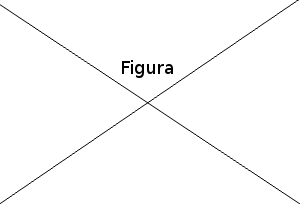
\includegraphics[scale=0.5]{figuras/temp.png}
\caption{Método das diferenças Finitas e método dos Elementos Finitos}
\label{fig:mdfFem}
\end{figure}

Diferentemente do MDF, como coloca \cite[p. 4]{huebner}, o MEF divide o domínio não em pontos, mas em subdomínios sobre os quais as equações são aproximadas por partes, e não pontualmente, como ocorre no MDF. O FEM também é capaz de representar mais fielmente o contorno (ou a borda) do problema. Desta forma, ele se apresenta como uma técnica mais poderosa e versátil para a modelagem de fenômenos com geometria complexa e meios não homogêneos \cite[p. 390]{sadiku}. 

O MEF surgiu originalmente como uma técnica de análise de deslocamentos e elasticidade de estruturas mecânicas, mas em seguida foi estendido para solucionar problemas de outros campos da física e da engenharia \cite[p. 19]{jin} \cite[p. 3]{desai} \cite[p. 2]{zien}

As primeiras formulações do MEF são conhecidas como \textbf{abordagem direta} ou \textbf{formulação física}, que embora forneça a interpretação intuitiva do método, é util apenas para a resolução de problemas relativamente simples \cite[p. 6]{huebner}. O uso do princípio do trabalho virtual, para a determinação de forças na abordagem direta, levou à generalização do MEF, por meio da estratégia de minimização do funcional de energia. Esta técnica mais genérica  ficou conhecida como \textbf{formulação Variacional} \cite[p. 113]{desai} \cite[p. 20]{zien}. Uma terceira abordagem, conhecida como \textbf{Método dos Resíduos Ponderados} ou \textbf{MEF generalizado} \cite[p. 61]{zien} é tradicionalmente utilizada e é ainda mais genérica que o princípio Variacional, pois resolve diretamente as equações diferenciais do modelo, sem necessitar da existência de um funcional \cite[p. 261]{desai}. Neste trabalho será adotado o método dos resíduos ponderados, mais especificamente, o método de Galerkin.


\subsection{Sistema de Elementos Discretos}
\cite[p. 68]{desai} introduz o conceito de Método de Elementos Discretos (MED) como sendo uma etapa intermediária da formulação física MEF. Na representação em elementos discretos, cada elemento é unidimensional, de tal forma que o sistema completo é representado por uma estrutura aramada, conforme mostra a figura \ref{fig:arame}.

De forma similar, \cite[p. 2]{zien} apresenta o Sistema Discreto Padrão (SDP) como uma forma unificada de analisar problemas de natureza discreta.

Em ambos os casos, os sistemas originais não se tratam de um contínuo, propriamente dito, mas de um sistema composto por partes, no entanto, são muito úteis na compreensão do funcionamento do MEF e do conceito de elemento.


\begin{figure}[!htb]
\centering
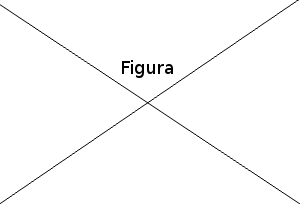
\includegraphics[scale=0.5]{figuras/temp.png}
\caption{Estruturas aramadas idealizadas}
\label{fig:arame}
\end{figure}





\subsection{Etapas de Processamento}
A computação de um problema modelado a partir de elementos finitos compreende basicamente três etapas: 
\begin{enumerate}  
\item \textbf{Pré-processamento}: Entrada de Dados ou discretização;
\item \textbf{Processamento}: Análise do problema e  solução do sistema de equações;
\item \textbf{Pós-processamento}: Apresentação dos Resultados. 
\end{enumerate}

Cada etapa apresenta uma contribuição para que se obtenha um resultado satisfatório. O pré-processamento é responsável pela discretização e por estabelecar as restrições físicas do domínio. A etapa de análise obtém a aproximação do modelo (forma fraca), e aplica esta aproximação em cada sub-domínio. O resultado preliminar da análise é um sistema de equações lineares que quando resolvido, fornece a solução do problema.  O pós-processamento consiste na exibição adequada dos resultados \cite[p. 665, 666]{zien}.


Nas seções a seguir cada etapa é vista em detalhes.

\section{Pré-Processamento}

A etapa de pré-processamento compreende a maior parte do tempo de modelagem do método. É neste ponto do processo que se são definidos os apectos geométricos do modelo, as propriedades dos materiais do objeto em análise e a aplicação das condições de contorno \cite[p. 9, 665]{zien}

\subsection{Aspectos geométricos} 
A definição dos aspectos geométricos consiste na tranformação do domínio contínuo $\Omega$ em uma malha de elementos finitos. Cada elemento $\Omega_e$ dessa malha será tratado como um subdomínio de $\Omega,$.  
Nesta etapa são definidas a forma, o número e o tamanho dos elementos, de forma que a representação seja a mais próxima possível do objeto em análise \cite[p. 154]{desai}.
A figura \ref{fig:elementos} contém a representação de elementos tipicamente utilizados em 1, 2 e 3 dimensões. 

\begin{figure}[!htb]
\centering
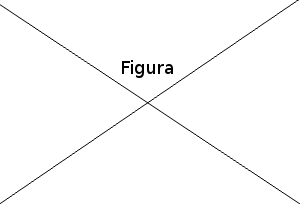
\includegraphics[scale=0.5]{figuras/temp.png}
\caption{Elementos em 1, 2 e 3 dimensões}
\label{fig:elementos}
\end{figure}

Conforme pode ser visto na figura \ref{fig:numeracao}, cada elemento pode ser identificado na malha a partir de um número que lhe é atribuído. De forma similar, os vértices (ou nós) também são numerados. Cada nó possui dois valores vinculados a ele. 
O primeiro número de cada par ordenado representa a numeração global nó, ou seja, a identificação do nó na malha. O segundo número do par ordenado é a numeração do nó dentro de um dado elemento (Identificação local). A numeração local é geralmente feita no sentido anti-horário, a fim de se obter um valor positivo no cálculo da área ou volume por meio do  determinante \cite[p. 394]{sadiku}. 

Um fator que deve ser levado em consideração é o balanceamento entre o refinamento da malha e o esforço computacional necessário \cite[p. 154]{desai}. Como o valor da solução é aproximado para cada elemento, o excesso de elementos pode causar a propagação do erro de aproximação, levando a resultados indesejáveis.


\begin{figure}[!htb]
\centering
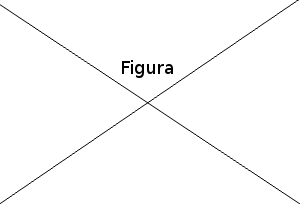
\includegraphics[scale=0.5]{figuras/temp.png}
\caption{Identificadores de Elementos e nós}
\label{fig:numeracao}
\end{figure}

\subsection{Propriedades do material}
Para que o MEF seja capaz de aproximar adequadamente a solução de um problema, é necessário, além da geometria, se especificar as propriedades do material de cada elemento da malha, sobretudo em meios não homogêneos. Na análise estrutural, por exemplo, aspectos como a plasticidade, elasticidade e porosidade podem afetar os resultados \cite[p. 250]{desai}. Já na análise eletromagnética, algumas propriedades relevantes são a condutividade ($\sigma$), permeabilidade ($\mu$) e a permissividade ($\epsilon$) \cite[p. 3]{volakis}. Na análise térmica algumas propriedades importantes são o calor específico e a condutividade térmica \cite[p. 251]{desai}.
Desta forma, de acordo com a área de análise, os materiais apresentam características determinantes para a obtenção de resultados adequados.

As propriedades dos materiais podem ainda estar condicionadas à uma determinada direção. Desta forma, os materiais podem ainda ser classificados como isotrópicos ou anisotrópicos\cite[p. 20]{sadiku}.  Materiais isotrópicos apresentam as mesmas propriedades físicas em todas as direções. Nos materiais anisotrópicos, as propriedades variam conforme a direção considerada.

Fenômenos eletromagnéticos dependem adicionalmente da linearidade do meio. Meios lineares são aqueles em que a condutividade, a permeabilidade e a permissividade independem da intensidade do campo elétrico e do campo magnético \cite[p. 20]{sadiku} .


\subsection{Valores de Contorno}
A atribuição dos valores de contorno é o último passo da etapa de pré- processamento. Estes valores são atribuídos a pontos específicos da malha e são importantes para caracterizar a unicidade de solução \cite[p. 7]{zien}

Considere um capacitor de placas paralelas, no qual uma das armaduras é submetida à uma tensão de 10V e outra à 0V. A ditribuição de potencial e o valor do campo elétrico entre as placas e no ambiente em volta do capacitor, podem ser definidos unicamente a partir das condições de contorno (10V e 0V) impostas em pontos (ou nós) específicos do domínio, como mostra a figura \ref{fig:capacitor}.

\begin{figure}[!htb]
\centering
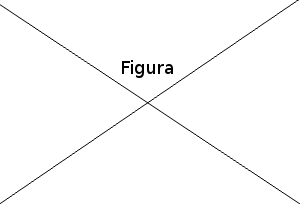
\includegraphics[scale=0.5]{figuras/temp.png}
\caption{Distribuição do potencial e o campo elétrico no capacitor de placas paralelas}
\label{fig:capacitor}
\end{figure}


\section{Processamento ou Análise de Elementos Finitos}
A etapa de processamento do MEF consiste basicamente em 3 passos \cite[p. 31]{jin}:

\begin{enumerate}  
\item Seleção das funções de interpolação;
\item Formulação do sistema de equações;
\item Solução do sistema de equações. 
\end{enumerate}

Cada um dos passos acima serão brevemente apresentados nesta seção, mas dada a sua importância e amplitude, eles serão aprofundados nas seções seguintes.

\subsection{Seleção das funções de interpolação}
O primeiro passo na etapa de processamento é a escolha de uma função de interpolação (função de base ou função de forma) \cite[p. 37]{volakis} que fornece uma aproximação da equação em cada elemento \cite[p. 32]{jin}. 
A função interpoladora escolhida geralmente é um polinômio, e isso ocorre por dois motivos a priori: \cite[p. 77]{desai}

\begin{itemize}  
\item Facilidade de manipulação matemática, principalmente derivação e integração;
\item Aproximação satisfatória quando truncado em uma ordem qualquer.
\end{itemize}

Na prática são escolhidos polinômios de primeira ou segunda ordem, mas ordens superiores podem ser adotadas para reduzir o erro de aproximação, no entanto, ocorre também o aumento da carga computacional \cite[p. 32]{jin}.

Sendo $N$ a função interpoladora, a solução aproximada $\tilde{\phi}$ para cada um dos $n$ nós de um dado elemento $e$ pode ser dada como:

 \begin{equation}
    \label{eq:interpol}
        \tilde{\phi^e} = \sum_{j=1}^{n}{N_j^e \phi_j^e} = 
        \{N^e\}^T \{\phi^e\} = \{\phi^e\}^T \{N^e\}
 \end{equation}

Neste caso, $N_j^e$ é a função de forma do nó $j$ no elemento $e$ e $\phi_j^e$ é o valor de $\phi$ no nó $j$ do elemento $e$.
Uma característica importante a ser obervada nas funções $N_j^e$ é que elas são diferentes de zero apenas sobre o subdomínio $e$.

\subsection{Formulação do sistema de equações}
Métodos variacionais ou de resíduos ponderados são tradicionalmente utilizados para se obter um sistema de equações que satisfaça um modelo diferencial \cite[p. 34]{jin}. No modelo de elementos discretos apresentado anteriormente, o sistema de equações existe naturalmente.

Na abordagem variacional destaca-se o método de Ritz, ou Rayleigh-Ritz, o qual tem por objetivo, minimizar o funcional variacional, ou funcional de energia, do problema aproximado \cite[p. 24]{volakis}. Embora tal abordagem tenha sido historicamente utilizada e possua fundamentação física e matemática, sua adoção, em muitos casos, é mais complicada em relação ao Método dos Resíduos Ponderados, pois demanda a formulação variacional do problema. Desta forma, se um problema é dado por um modelo diferencial, é necessário se obter a partir deste modelo a forma variacional equivalente, para só então se aplicar o método para a obtenção do sistema de equações. No eletromagnetismo, a formulação variacional das equações de Maxwell não é bem estabelecida \cite[p. 211]{jin}.

Para problemas que apresentam explicitamente condições de Dirichlet no contorno e cujo operador $\mathcal{L}$ é linear e auto-adjunto, é possível se obter imediatamente o funcional (ou forma variacional) \cite[p. 81]{zien}, no entanto, como mostra \cite[p. 29]{volakis}, a mesma integral da formulação variacional é obtida pelo método de Galerkin.

\subsubsection{O método dos resíduos ponderados}

Seja a equação \ref{eq:operador}, uma equação diferencial que modela um determinado fenômeno físico, na qual $\mathcal{L}$ é um operador diferencial, $f$ é uma função de excitação conhecida e $\phi$ é a solução procurada \cite[p. 20]{jin}\cite[p. 24]{volakis}.

 \begin{equation}
    \label{eq:operador}
    \mathcal{L} \phi = f
 \end{equation}
 
 Se substituirmos a solução exata pela sua aproximação apresentada na equação \ref{eq:interpol}, um resíduo $r$ surge, como pode ser visto na equação \ref{eq:residuos}, em decorrencia dos erros de aproximação.
 
  \begin{equation}
    \label{eq:residuos}
    r = \mathcal{L} \tilde{\phi} - f \neq 0
  \end{equation}

Como não se pode requerer que os resíduos da aproximação seja zero sobre todo o domíno $\Omega$ (o que ocorre na solução exata), faz-se a aproximação ou poderação dos resíduos em cada subdomínio $e$, como mostram as equações \ref{eq:res1} e \ref{eq:res2}. Desta forma, na média, a condição residual é atendida \cite[p. 28]{volakis}

  \begin{equation}
    \label{eq:res1}
    R_i = \int_{\Omega}{w_i r \ d\Omega} = 0
  \end{equation}
  
  \begin{equation}
    \label{eq:res2}
    R_i = \int_{\Omega}{w_i [\mathcal{L} \tilde{\phi} - f] \ d\Omega} = 0
  \end{equation}  


A escolha particular de $w_i = \phi_i$ configura o método de Galerkin, o qual, para um operador $\mathcal{L}$ auto adjunto, fornece o mesmo resultado que o método de Ritz  \cite[p. 22]{jin}, conforme a seguinte equação

  \begin{equation}
    \label{eq:galerkin}
    R_i = 
    \int_{\Omega}{N_i \mathcal{L} \{N\}^T \{\phi\} \ d\Omega\}} - \int_{\Omega}{N_i f \ d \Omega} = 0
  \end{equation}  
  
  
  o Resultado da equação \ref{eq:galerkin} é um sistema esparso de equações lineares, representado na equação \ref{eq:sistema}. Se o operador diferencial for auto-adjunto, o sistema é simétrico \cite[p. 36]{volakis}.
  
    \begin{equation}
        \label{eq:sistema}
        [K]\{\phi\} = {b}
    \end{equation}  

É importante colocar que o parâmetro $w_i$ deve ser um conjunto de funções integraveis, linearmente independentes
\cite[p. 60]{reddy}. Alguns casos especiais do método dos resíduos ponderados são obtidos a partir da escolha de $w_i$:

\begin{equation}
\label{eq:metPond}
    \begin{tabular}{ l l }
    Método de Petrov-Galerkin & $ w_i = \psi_i \neq \phi_i $ \\ 
    Método de Galerkin & $ w_i = \phi_i $\\  
    Método dos Mínimos quadrados & $ w_i = \frac{d}{dx} \left(a(x)\frac{d \phi_i}{dx}\right) $ \\ 
    Método da colocação & $ \delta(x - x_i)  $ 
    \end{tabular}
\end{equation}



\paragraph{Funções sobre o espaço discreto \\}

Nesta seção será apresentada a visão geral do método. Para tal, os conceitos de formulação forte e fraca não serão necessários, visto que os problemas aqui descritos são modelados por sistemas lineares e não por equações diferenciais. Assim sendo, o MEF pode ser aplicado diretamente ao problema, sem a necessidade de se obter a forma integral (forma fraca) a partir de técnicas à relaxação da forma forte, como por exemplo o princípio dos trabalhos virtuais (abordagem direta), o método de Ritz (abordagem Variacional) e de Galerkin (abordagem por Resíduos ponderados).

Considere a malha bidimensional  apresentada na figura \ref{fig:malhaGenerica}. Esta malha pode representar por exemplo, a abstração de uma ponte metálica, de dutos de um fluido ou até mesmo um circuito elétrico, como apresentado na figura \ref{fig:repMalhaGenerica}.
\begin{figure}[!htb]
\centering
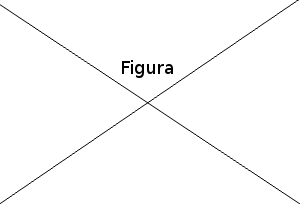
\includegraphics[scale=0.5]{figuras/temp.png}
\caption{Malha Genérica}
\label{fig:malhaGenerica}
\end{figure}

\begin{figure}[!htb]
\centering
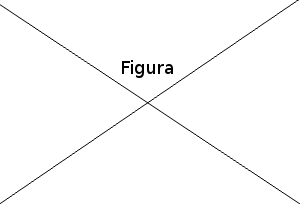
\includegraphics[scale=0.5]{figuras/temp.png}
\caption{Possíveis objetos de representação da malha \ref{fig:malhaGenerica}}
\label{fig:repMalhaGenerica}
\end{figure}


 Fazendo uma analogia com uma estrutura metálica, conforme apresentado na figura \ref{fig:repMalhaGenerica}-a, as forças que atuam nos nós, podem ser definidas  a a partir dos deslocamento destes nós, da distribuição da carga sobre um dado elemento e da tensão inicial, caso haja.
 
 Supondo que um carregamtno $p$ atue sobre o elemento $1$, as forças que atuam sobre os nós deste elemento podem ser dadas por:
 
 
 \begin{equation}
    \label{eq:forca}
    \begin{tabular}{c c}
    $q_1 = 
        \left \{
        \begin{tabular}{c}
            $q_1^1$ \\
            $q_2^1$ \\
            $q_3^1$
        \end{tabular}       
        \right \}$
        \
    $q_1^1 = 
        \left \{
        \begin{tabular}{c}
            $U_1$ \\
            $V_1$
        \end{tabular}       
        \right \}   $
        \end{tabular}   
 \end{equation}


Similarmente, os deslocamentos podem ser dados para cada nó do elemento. Se as componentes da força na direção de x e y são dadas como U e V, as componentes da força podem ser dadas em função dessas componentes de deslocamento.

 \begin{equation}
    \label{eq:desloc}
    \begin{tabular}{c c}
    $u_1 = 
        \left \{
        \begin{tabular}{c}
            $u_1^1$ \\
            $u_2^1$ \\
            $u_3^1$
        \end{tabular}       
        \right \}$
        \
    $u_1^1 = 
        \left \{
        \begin{tabular}{c}
            $u_1(U_1)$ \\
            $v_1(V_1)$
        \end{tabular}       
        \right \}   $
        \end{tabular}   
 \end{equation}


Assumindo um material isotrópico, cujo comportamento é linear elástico, a lei de Hooke fornece a equação \ref{eq:hooke}

 \begin{equation}
    \label{eq:hooke}
    \textbf{$q^1 = K^1 u^1 + f^1$}
 \end{equation}
 
 O vetor $q$ representa as forças induzidas pelos deslocamentos $u$ dos nós. A matriz $K$ é a matriz de rigidez ou matriz de coeficientes do problema. $f$ é a força ou tensão inicial do elemento. Caso o estado inicial do elemento seja de equilíbrio, $f$ é igual a zero.
 
 Para que a representação seja adequada é necessário que sejam estabelecidas condições de compatibilidade de deslocamentos e equilíbrio.
 
 A compatibilidade de deslocamento é necessária, uma vez que quando um nó de um elemento é deslocado em uma direção, os elementos vizinhos que compartilham o mesmo nó também são afetados com este deslocamento. Esta condição é satisfeita aos se relacionar todas as forças do sistema.
 
 \paragraph{Montagem do Sistema Global}
 
 Para que o conjunto de funções de força ou tensão sobre os subdomínios sejam corretamente agregadas em um sistema global, é necessário se estabelecer as condições de compatibilidade de deslocamento e de equilíbrio.
 
 Como um nó de um elemento é compartilhado com os elementos vizinhos, a compatibilidade dos deslocamentos ocorre por meio da montagem de um sistema global. Este sistema possibilita que todos os deslocamentos estejam relacionados entre si.
 
  A figura \ref{fig:loc2glob} mostra a transformação dos sistemas locais para um sistema com referências globais. Como todos os nós são relacionados entre si, a matriz de rigidez é quadrada e também simétrica para o caso de materiais isotrópicos.
  
  \begin{figure}[!htb]
  \centering
  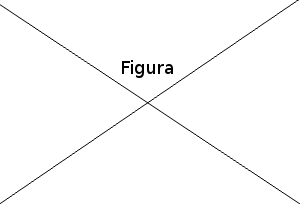
\includegraphics[scale=0.5]{figuras/temp.png}
  \caption{}
  \label{fig:loc2glob}
  \end{figure}
  
  O sistema em \ref{eq:assembly} mostra a relação entre todos os pontos do domínio para um dado elemento. é importante notar que apenas elementos adjacentes se afetam mutuamente.
  
 \begin{equation}
    \label{eq:assembly}
    \begin{tabular}{c c c}
    $q^e = 
        \left \{
        \begin{tabular}{c}
            $q^e_1$ \\
            $q^e_2$ \\
            \vdots \\
            $q^e_m$
        \end{tabular}       
        \right \}$
        \
    $u^e = 
        \left \{
        \begin{tabular}{c}
            $u_1$ \\
            $u_2$ \\
            \vdots \\
            $u_m$
        \end{tabular}       
        \right \}   $
        \
        $K^e =
        \begin{bmatrix}
            K^e_{11}    & K^e_{12}  & \dots     & K^e_{1m} \\
            K^e_{11}    & \ddots  & \   & \vdots \\
            \vdots  & \vdots     & \    & \vdots \\
            K^e_{m1}    & \dots   & \dots   & K^e_{mm} 
        \end{bmatrix}    $      
    \end{tabular} 
 \end{equation}
 
 Com os deslocamento relacionados em todos os pontos elementos do sistema,
 a condição de equilíbrio é satisfeita quando o somatório das forças causadoras de tais deslocamentos nula, ou seja, a resultante em um dado ponto $a$ vale zero.
 
  \begin{equation}
    \label{eq:somaForcas}
    \sum_{e=1}^{m}{q_a^e = q_a^1 + q_a^2 + \dots = 0}
  \end{equation}
  
  Considerando que o corpo está inicialmente em equilíbrio, ou seja, $f = 0$, o sistema como um todo pode ser representado como 
  
    \begin{equation}
        \label{eq:equilibrio}
        q =
        \sum_{b=1}^{n}\sum_{e=1}^{m}{K_{ab}^e u_b = 0}
    \end{equation}
    
    
\paragraph{Atribuição das condições de Contorno \\}
A atribuição dos valores de contorno da variável $u$ consiste na especificação dos deslocamentos ou deformações prefixadas no sistema. No exemplo \ref{fig:repMalhaGenerica}-a, como análise estrutural, as condições de contorno podem ser os deslocamentos nulos impostos nós fixados (soldados) ou condições iniciais de tensão ou torção. a equação \ref{eq:condIni} exemplifica a atribuição dessas condições.

\begin{equation}
    \label{eq:condIni}
    u_1 = u_6 = 
        \left \{
        \begin{tabular}{c}
            $0$ \\
            $0$ \\
        \end{tabular}       
        \right \}   
\end{equation}

A inserção de valores de contorno no sistema promove a redução do número de equações de equilíbrio, por meio da eliminação das linhas cujo valor de $u$ já foi especificado.

\paragraph{Exemplo \\}

A fim de exemplificar a etapa de processamento,  considere a malha de resistores introduzidas  em \ref{fig:repMalhaGenerica}-b. Neste caso, as condições de contorno são as a tensões fornecidas por uma bateria.

\subsubsection{Pós-Processamento}
A etapa de pós processamento consiste na apresentação dos resultados obtidos no processamento e na determinação de variáveis secundárias a partir destes resultados.

A apresentação da solução pode ser feita graficamente por diferentes técnicas, como curvas de nível, mapas vetoriais, sobreposição de imagens e animações. Alguns exemplos são dados na figura \ref{fig:graf}

\begin{figure}[!htb]
\centering
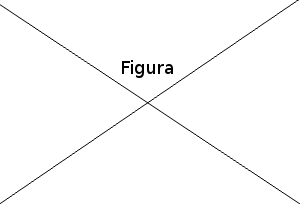
\includegraphics[scale=0.5]{figuras/temp.png}
\caption{}
\label{fig:graf}
\end{figure}

Com base nos valores apresentados no pós processamento, novas decisões são tomadas, tanto para otimizar os resultados quanto para melhorar a performance.

\subsection{Abordagem Direta \\}

A abordagem direta, abordagem física ou formulação de deslocamentos foi a primeira tentativa de se modelar um problema físico em termos de elementos finitos.

Voltada para a análise de estruturas e problemas de elasticidade, esta técnica busca aproximar o comportamento de um problema contínuo, por meio de elementos finitos, que se comporte de maneira similar a elementos reais discretos.
\cite[p. 19]{zien}

A partir desta abordagem, a forma fraca do problema diferencial é obtida com o uso do princípio dos trabalhos virtuais.
\cite[p. 20]{zien}

 






% ---
% Capítulo da implementação da proposta
% ---
\chapter{Procedimentos metodológicos}
% ---
Para o desenvolvimento deste trabalho foi tomado como base uma sequência de etapas que envolveram desde o estudo e compreensão dos conceitos de AG até o desenvolvimento e adaptação do mesmo para o alcance do objetivo proposto.


\chapter{Implementação}
\label{chap:implementacao}

Neste capítulo está descrito a forma que foi implementado a proposta deste trabalho, a modelagem da população e os operadores genéticos. Assim como, as duas implementações de AG.


\begin{algorithm}
    \caption{\label{fga} Pseudocódigo FGA} 
    \begin{algorithmic}[1]
        \State{Definir valores das variáveis: $quantidadeDeFunções$ e $quantidadeDeGerações$;}
        \For{ $função$\_$n$ }{ 0}{ até }{$quantidadeDeFunções$}
        \State {Gerar população inicial com valores aleatórios no intervalo da função corrente ($função$\_$n$);}
        \State {Avaliar população inicial com a função corrente} ($função$\_$n$);
    \For{$geração$}{ 1}{ até }{$quantidadeDeGerações$}
    \State {Gerar população de filhos por recombinação  \textit{crossover} aritmético;}
    \State {Avaliar população de filhos com a função corrente;}
    
    \State {Gerar população de mutante por mutação gaussiana;}
    \State {Avaliar população de mutantes com a função corrente;}
    
    \State {Concatenar: população inicial + população de filhos + população mutados;}
    
    \State{Ordenar população concataneda;}  
    \State {Selecionar 20\% dos indivíduos por elitismo, em relação ao tamanho da população inicial;}
    \State {Selecionar 80\% pelo método \textit{roullete wheel}, em relação ao tamanho da população inicial;}
    \State{Substituir na população incial os inivíduos selecionados;}
    \EndFor
    \EndFor
\end{algorithmic}
\end{algorithm}


% ---
% Capítulo dos Resultados
% ---
\chapter{Resultados}
Os resultados apresentados e analisados nesta seção, tratam-se dos \textit{fitness} resultantes das funções objetivo utilizadas, a fim de comparar as implementações propostas neste trabalho, investigando então, o uso da regra de um quinto de sucesso aplicado no operador de \textit{crossover}. 


% ----------------------------------------------------------
% Finaliza a parte no bookmark do PDF
% para que se inicie o bookmark na raiz
% e adiciona espaço de parte no Sumário
% ----------------------------------------------------------
\phantompart

% ---
% Conclusão
% ---
\chapter{Conclusão}
% ---

Concl

% ----------------------------------------------------------
% ELEMENTOS PÓS-TEXTUAIS
% ----------------------------------------------------------
\postextual
% ----------------------------------------------------------

% ----------------------------------------------------------
% Referências bibliográficas
% ----------------------------------------------------------
\bibliography{abntex2-modelo-references}
%\bibliography{bibfile}

% ---
% Inicia os apêndices
% ---
\begin{apendicesenv}
\label{chap:apendices}

% Imprime uma página indicando o início dos apêndices
\partapendices

% ---
\chapter{Tabelas do primeiro teste}
apendice

% ---


\end{apendicesenv}
% ---

\end{document}
